%%% File: ./inputs/parts/ACTION_SELECTION.tex

%%% %%%%%%%%%%%%%%%%%%%%%%%%%%%%%% BEGIN COMPLEMENTARY MEMORY %%%%%%%%%%%%%%%%%%%%%%

%%% Solves the problem of initializing / allocating networks that 
%%% span the input space, but that are unlikely to interfere with 
%%% one another and can be gradually integrated with other systems. 

%%%%%%%%%%%%%%%%%%%%%%%%%%%%%%%%%%%%%%%%%%%%%%%%%%%%%%%%%%%%%%%%%%%

In both neuroscience and artifial intelligence, reinforcement learning problems are typically modeled as Markov decision problems (MDPs). While MDPs can be solved in polynomial time, the size of the state space is often prohibitively large, making practical solution intractable~\cite{LittmanetalUAI-95}. Hierarchical reinforcement learning offers a means of reducing the computational burden by decomposing the state space resulting in a relatively small number of tractable MDPs each of which can be solved independently~\cite{KaelblingICML-93,DietterichJAIR-00,HengstEMLDM-17}. However, the problem of finding an optimal decomposition is itself intractable and hence it is necessary to resort heuristic methods and approximate solutions.

There exist a number of approaches that develop solutions to the problem of hierarchical reinforcement learning (HRL) employing various decomposition strategies, several of which we draw inspiration from~\cite{NarasimhanetalJAIR-18,AndreasetalICML-17,SahnietalCoRR-17,KulkarnietalNIPS-16,BakkerandSchmidhuberIAS-04,MoffaertandNoweJMLR-14,PashevichetalCoRR-18} including a few that relate to biological or biologically plausible models~\cite{RasmussenetalPLoS-ONE-17,DiuketalCRMHOB-13,FrankandBadreCEREBRAL-CORTEX-12,RibasFernandesNEURON-11}. It's important to keep in mind that we are dealing a partially-observable, high-dimensional, continuous state space, and an action space that includes abstract cognitive activities in addition to concrete physical activities that engage the motor system in interacting with the environment. 

In the treatment here, we emphasize the problem of life-long learning as it relates to the nonstationarity of underlying process as a consequence of changes in the external environment and changes in the goals of the agent and the neural substrate available for computation during development and extending on into adulthood. In the case of a growing infant, the changes involve the appearance and maturation of critical circuits and the limitations of finite memory. In both human and machine, internal representations progress from concrete to abstract, building on a foundation grounded in the environment. This maturation in cognitive capability is accelerated by a curriculum that takes advantage of dependencies between concepts. 

%%%%%%%%%%%%%%%%%%%%%%%%%%%%%%%%%%%%%%%%%%%%%%%%%%%%%%%%%%%%%%%%%%%

%%% Figure~{\urlh{#fig_Hippocampus_Inspired_Learning_Redux}{\ref{fig_hippo}}}
\begin{figure}
%
  \begin{center} 
%    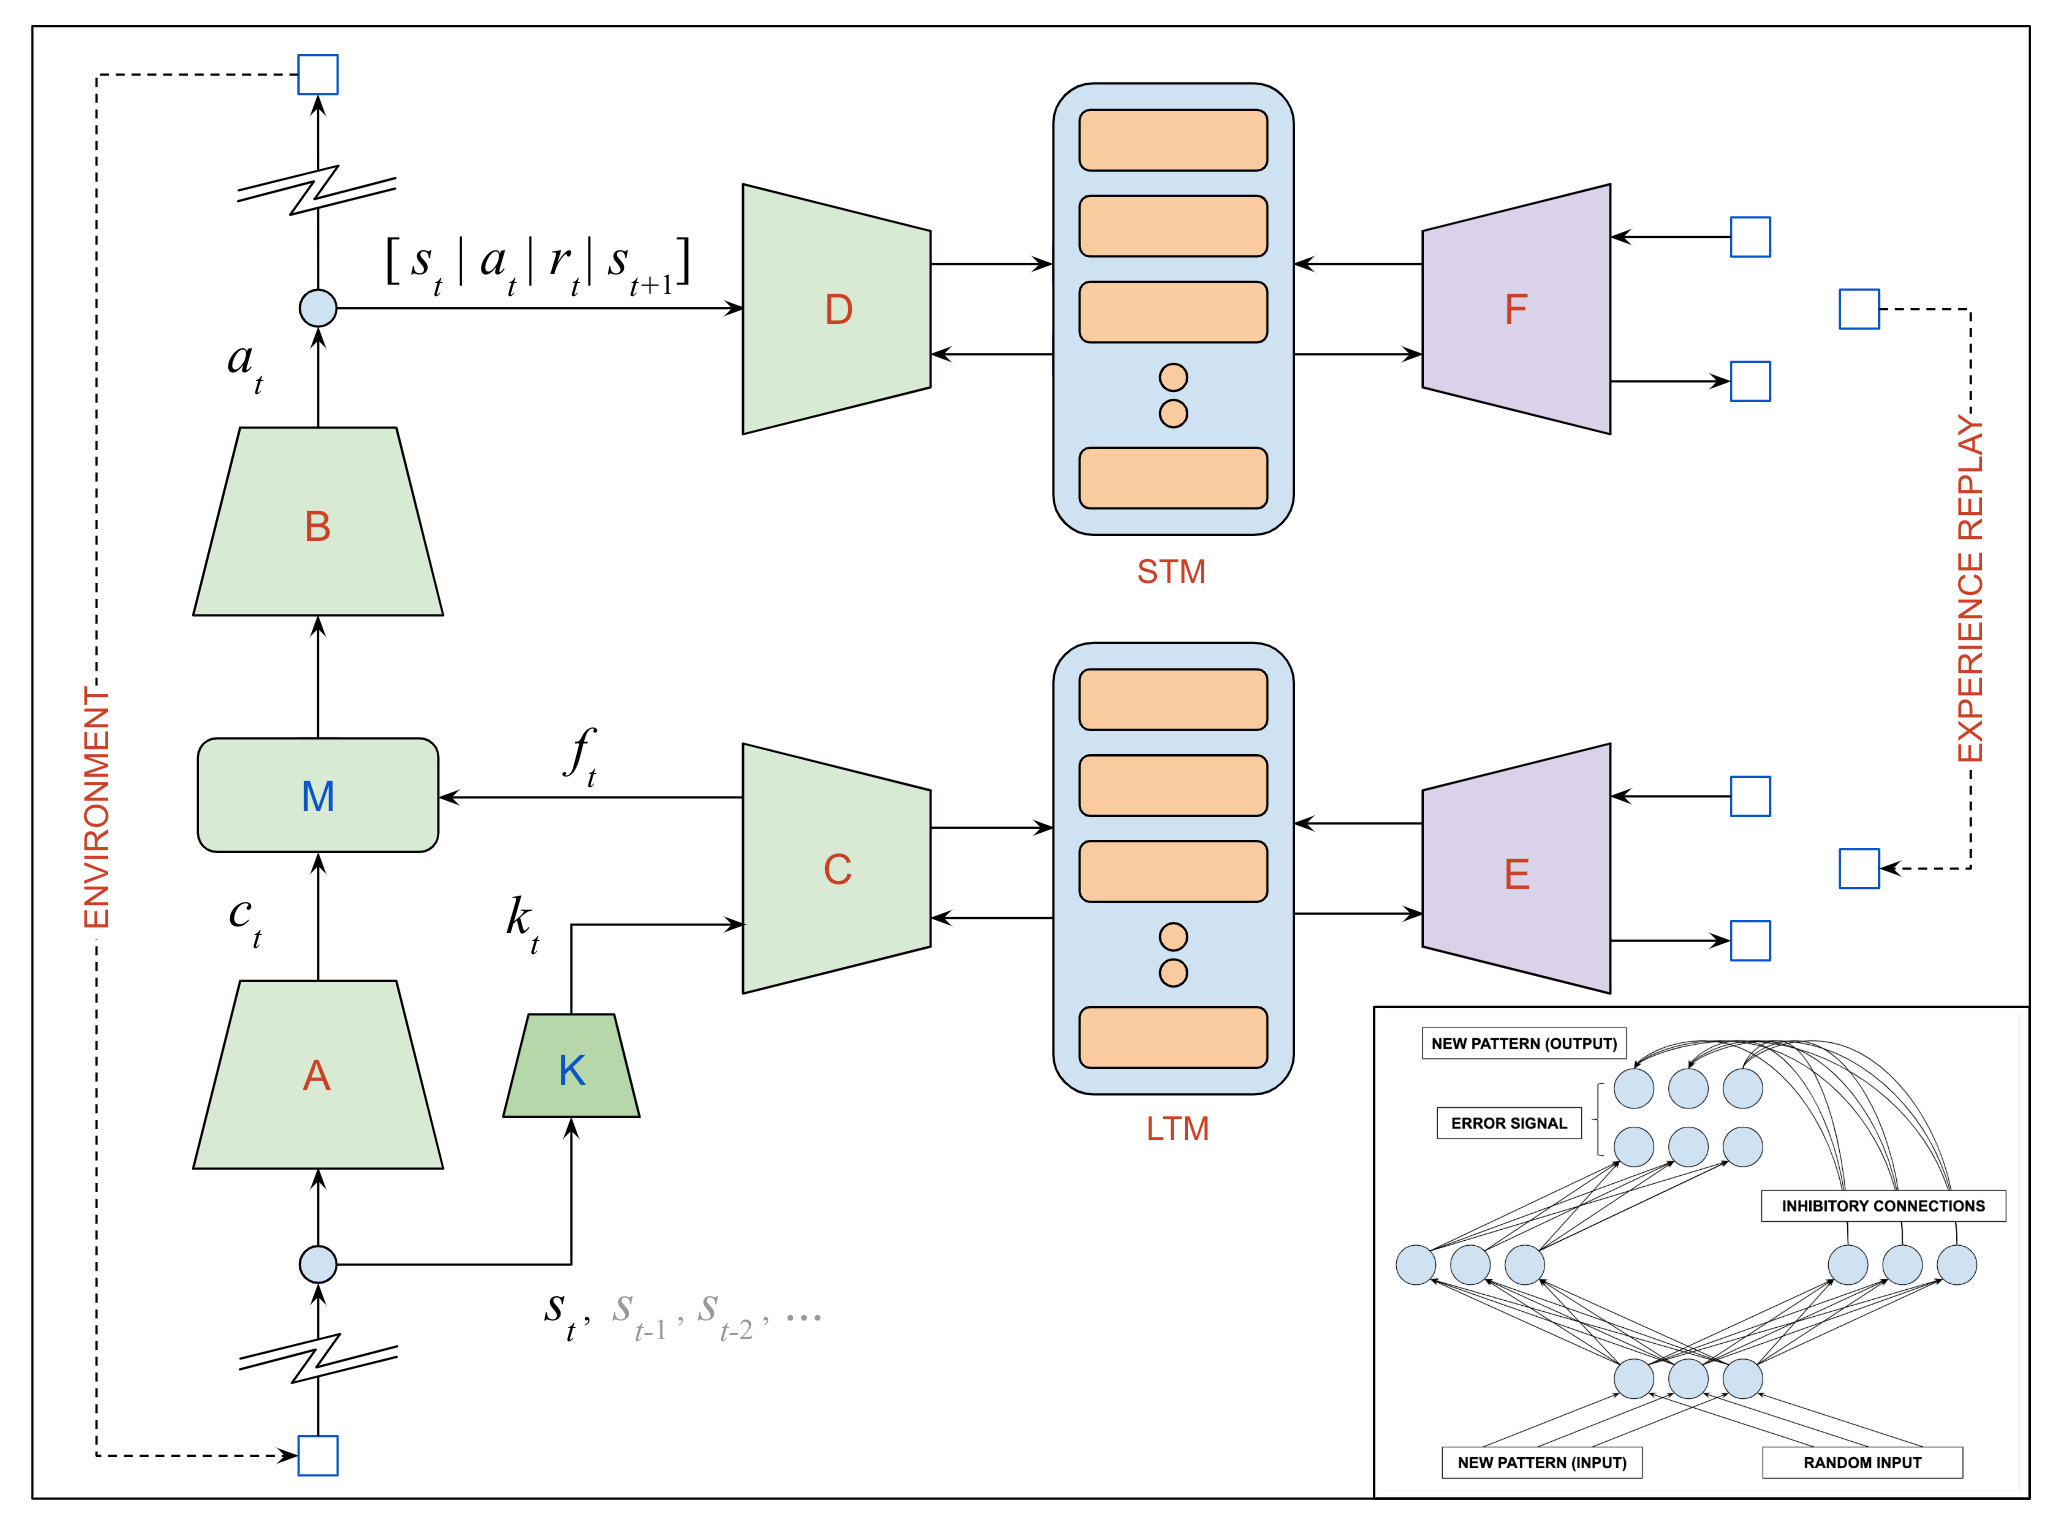
\includegraphics[width=700pt]{./figures/Hippocampus_Inspired_Learning_Redux.png} 
    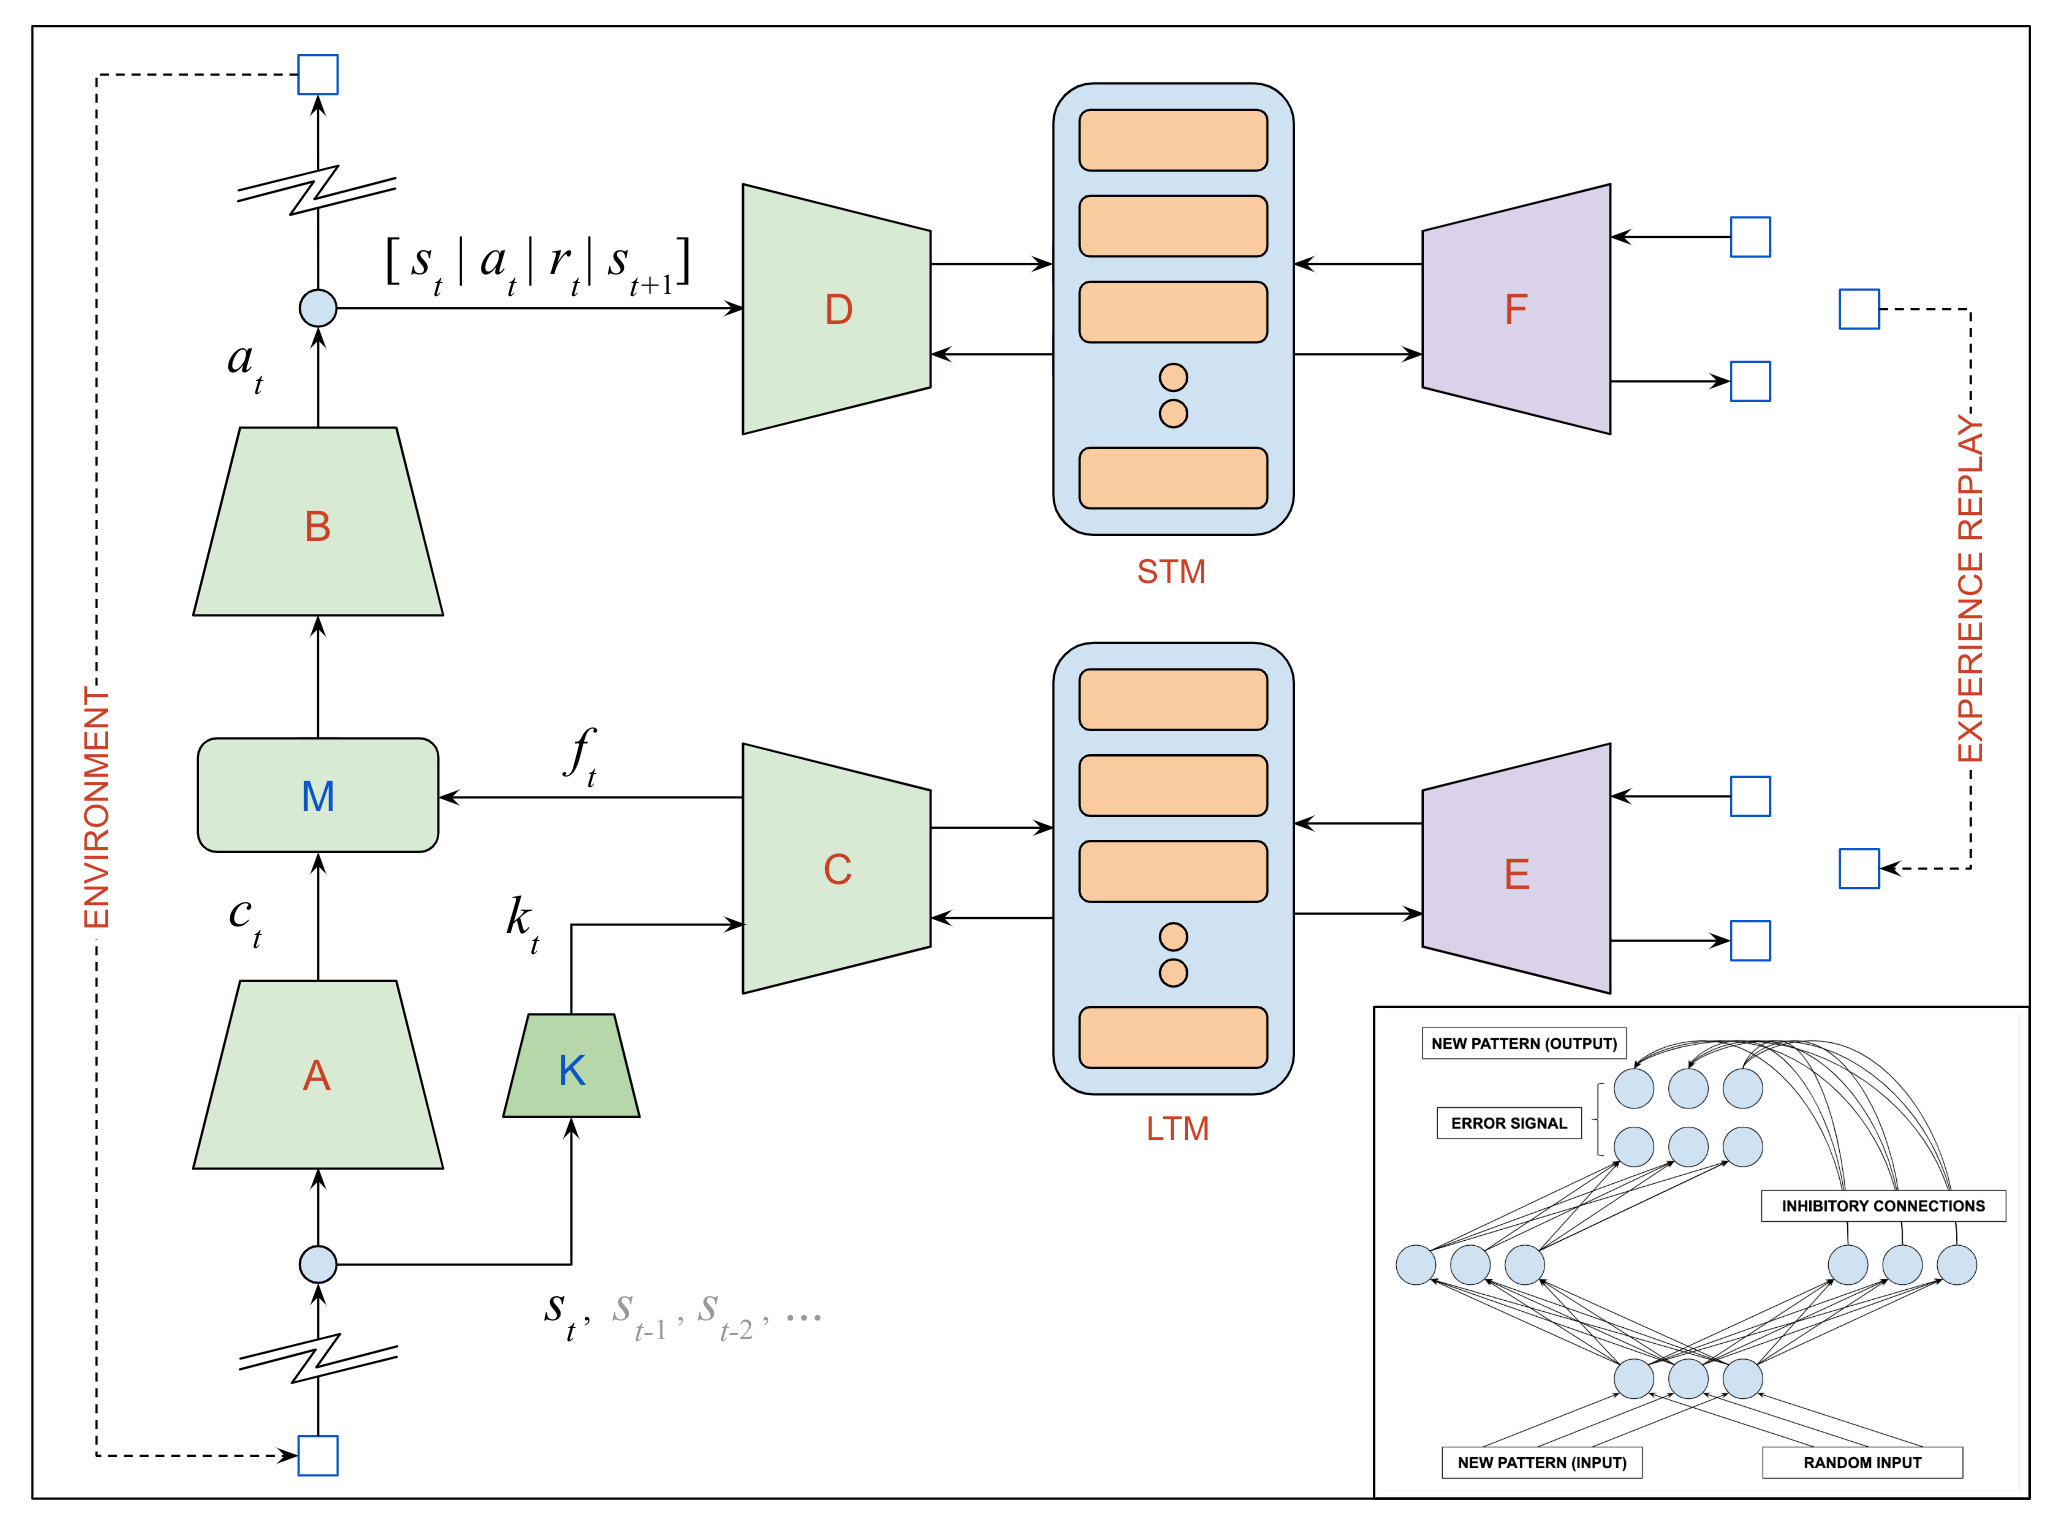
\includegraphics[width=350pt]{./figures/Hippocampus_Inspired_Learning_Redux.png} 
  \end{center}
%
  \caption{The network shown here takes as input a pattern of activation originating in the temporal and parietal lobes and selects an action to perform. The subnetworks labeled \colorred{A} and \colorred{B} are relatively straightforward multilayer neural networks that compute features and generate representations as their output. Network \colorred{A} takes as input a representation of the current state, and generates a representation of the context for action selection. Network \colorblu{K} is an embedding network that takes as input a sequence of states corresponding to recent activity and generates as output a unique key associated with a subspace of the full MDP state space that includes the current state. The box labeled \colorblu{M} corresponds to a location in working memory. The networks \colorred{C}, \colorred{D}, \colorred{E} and \colorred{F} are controllers for two differentiable neural computer (DNC) peripherals that provide storage and access for short-term and long-term memory respectively. The long-term memory is used to store the weights for networks that encode architecturally identical networks {\emdash{}} only the weights are different {\emdash{}} providing specialized expertise in restricted domains corresponding to subspaces of the full MDP state space. The model operates in two modes. In each cycle during the {\it{online mode}}, the \colorred{C} controller loads the selected expert network into location \colorblu{M} where it is fed the output of \colorred{A} and produces the input to \colorred{B}. In this mode, the short-term memory is used to record activity traces that are subsequently used in the {\it{offline}} mode to update the networks stored in long-term memory. The network in the lower-right inset implements a version of {\it{pseudo rehearsal}} as a means of mitigating catastrophic forgetting~\cite{FrenchTiCS-99}.}
%
  \label{fig_hippo}
%
\end{figure}

% %%%%%%%%%%%%%%%%%%%%%%%%%%%%%%%%%%%%%%%%%%%%%%%%%%%%%%%%%%%%%%%%%%%

The network model shown in Figure~{\urlh{#fig_Hippocampus_Inspired_Learning_Redux}{\ref{fig_hippo}}} illustrates a system that takes as input a pattern of neural activity originating in the medial temporal and inferior parietal cortex and selects an action to perform. This particular example is meant to illustrate how episodic memory might play an expanded role in action selection. For illustration, patterns of activity serve as proxies for the state of the external environment and are represented in the figure as a sequence $s_t, s_{t-1}, s_{t-2}, ...$. The subnetworks labeled \colorred{A} and \colorred{B} are relatively straightforward multilayer neural networks that compute features and generate representations as their output. Network \colorblu{A} takes as input a representation of the current state, and generates a representation of the {\it{context}} for action selection.

%%% In keeping with our objective to demonstrate how ideas from neuroscience can influence and accelerate the development of artificial intelligence, this model is not intended to emulate how the human brain processes information. Nor is the architecture intended to mirror that of the human brain or any other biological organism. What we borrow from neuroscience are ideas that enable engineers to solve problems that current AI systems cannot handle or do so poorly. We are not bothered by combining neural mechanisms that neuroscientists currently identify with, say, the basal ganglia with neural mechanisms associated with the hippocampal formation. At this stage in the development of more capable AI systems, what engineers need most are general principles that inform design and be applied whenever the need arises.

We'll explain the function of the box labeled \colorblu{M} in a moment; assume for now that it generates a representation of the options available for acting in the current context. Network \colorred{B} then takes these suggestions as input and produces as output a representation of the selected action. The boxes labeled \colorred{C}, \colorred{D}, \colorred{E} and \colorred{F} are controllers for two differentiable neural computer (DNC) units that provide storage and access for short-term and long-term memory respectively. The controllers on the left are part of the online system for selecting actions. The controllers on the right are responsible for off-line training during which the recorded actions, along with their associated states and rewards are consolidated in long-term memory using experience replay.

The blue boxes represent stored information in the form of key-value pairs. Each key is associated with a subset or {\it{subspace}} of the set of all states that represents a restricted domain of expertise for selecting actions. The value for this key is a function implemented as a network trained as an expert for the associated subspace. \colorblu{K} is an embedding network that takes as input a sequence of states corresponding to recent activity and generates as output a unique key associated with a subspace of the current state. A given state can belong to more than one subspace and the particular key selected at any given point in time depends on the current state and the immediately previous states in a fixed window. The order of the states matters. 

In the online phase, the embedding network retrieves this key which it forwards to the controller labeled \colorred{C} that uses it to retrieve the expert for the relevant subspace. The box labeled \colorblu{M} corresponds to a location in working memory and in each online cycle the \colorred{C} controller loads the expert subsystem in location \colorblu{M} of working memory where it can be utilized to compute a set of options appropriate for the current state. During off-line periods the system uses the recorded sequences of activity to run some variant of experience replay to update the relevant expert subsystems stored in long term memory~\cite{AndrychowiczetalCoRR-17,SchauletalCoRR-15,LinML-92}.

The training that occurs offline involves adjusting the weights of networks using relatively small samples and so runs the risk of catastrophic interference in transfer learning~\cite{McClellandetalPR-95}. One way in which we hope to ameliorate the adverse consequences of catastrophic interference is by defining separate networks for separate subspaces. The embedding space method mentioned in describing \colorblu{K} is designed to isolate expertise by identifying states that tend to occur together. The hope is that the actions exercised is such states will tend to be interrelated and hence they should be represented using the same network to facilitate their coordination. 

Of course temporal proximity in their occurrence doesn't guarantee they serve the same task since we are always getting distracted or interrupted requiring us to interleave tasks that have very little to do with one another. It may be possible to segment activity streams into coherent tasks in a similar way to how we segment conversations involving multiple speakers~\cite{SeldinetalICSS-01,SeldinetalICML-01}. Alternatively, there has been some success with the method of {\it{pseudo rehearsal}} which consists of retraining existing networks by interleaving new examples with synthetic-examples produced by randomly activating the existing network~\cite{ZhiyuanandBingLML-18,KirkpatricketalCoRR-16,AnsetalCSS-02,FrenchTiCS-99,FrenchCONNECTION-SCIENCE-97,RobinsCONNECTION-SCIENCE-95}.

In this model the STM roughly corresponds to the hippocampus as the storage system for episodic memory. The LTM resembles the cerebellum in the way that it essentially compiles prior activity to construct a set of programs each of which spans some portion of the overall state space. As described above, the STM is only used for temporary storage awaiting off-line replay to consolidate recent memories. An alternative is to maintain a much larger collection of episodic memories that can be used in a manner similar to that suggested in Gershman and Daw who posit that we routinely draw upon our stored memories in the hippocampus to figure out what to do in novel situations not covered by our other sources of procedural knowledge~\cite{GershmanandDawANNUAL-REVIEWS-17}. See {\urlh{box_memories}{Box~\colorred{B}}} for more detail concerning episodic memory and experience replay.

%%% %%%%%%%%%%%%%%%%%%%%%%%%%%%%%%%%%%%%%%%%%%%%%%%%%%%%%%%%%%%%%%%%%%%%%%%%%%%%

%%% File: ./inputs/boxes/BOX_MEGUMI_SANO.tex

\begin{center}
  %%% \begin{tcolorbox}[sharp corners=all,coltitle=black,colbacktitle=white,
  \begin{tcolorbox}[breakable,sharp corners=all,coltitle=black,colbacktitle=white,
    width=\textwidth,boxsep=5pt,left=5pt,right=5pt,
    title={\textbf{Box B: Replaying Experience, Consolidating Memory}}]

    %%% width=\textwidth,boxsep=5pt,left=5pt,right=5pt,hypertarget={box_memories},
    
~~~~When we encounter a new experience in the environment, we do not act independently of the past, but rather, our past experiences substantially inform our present decisions. Here, we introduce the basic principles of \textit{hippocampal replay} and a few key ways in which it has motivated reinforcement learning algorithms.

~~~~Replay is the process by which hippocampal representations of previous experiences are sequentially reactivated~\cite{CarretalNATURE-NEUROSCIENCE-11}. Studies show that cells in the rodent hippocampus replay past experiences to stabilize behaviorally relevant memories~\cite{OlafsdottirCURRENT-BIOLOGY-18,JooandFrankNATURE-REVIEWS-NEUROSCIENCE-18}. Though initially observed in spatial tasks, recent work suggests that non-spatial task states are also replayed, and that this phenomenon is common in humans~\cite{SchuckandNivDOI-18}. 

~~~~In the reinforcement learning literature, the \textit{experience replay} algorithm was introduced as an analogical framework in online learning agents~\cite{LinML-92}. Transitions containing state, action, and reward information are sequentially stored in memory and sampled randomly for learning. Randomly replaying old memories not only allows decorrelation of consecutive experiences encountered during data collection, but also enables reuse of training data, increasing sample efficiency, and encourages resampling of rare experiences, potentially alleviating forgetting. 

~~~~A relatively well-studied question is \textit{what to replay}. Some studies suggest the correlation of replay frequency with \textit{novelty} approximated by temporal difference (TD) error~\cite{FosterandWilsonNATURE-06}, and others with high \textit{reward}~\cite{OlafsdottirCURRENT-BIOLOGY-18}. In particular, dopaminergic release, which encodes both novelty and reward~\cite{MenegasetalELIFE-17}, enhances {\textit{sharp wave-ripple}} activation \emdash{} the basic unit of replay. Yet other studies show that experiences more \textit{vulnerable to forgetting} are more likely to be replayed~\cite{SchapiroetalNATURE-COMMUNICATIONS-18}. While the exact selection algorithm is unknown, the observed association with novelty inspired the \textit{prioritized experience replay} algorithm which samples experiences with probabilities weighted by their TD errors and is now consistently preferred to the originally proposed uniform sampling variant~\cite{SchauletalCoRR-15}. 

~~~~The significantly less studied question is \textit{what happens during replay}. Besides re-learning of experiences, many neuroscientists support the idea that replay also serves as a substrate for \textit{memory consolidation} \emdash{} the gradual integration of new experiences processed into existing knowledge representations in the neocortex~\cite{WilsonandMcNaughtonSCIENCE-94,McClellandetalPR-95,KarlssonandFrankNATURE-NEUROSCIENCE-09,BendorandWilsonNATURE-NEUROSCIENCE-12,KumaranetalTiCS-16}, as to stabilize memories against interference. The idea is that replaying information stored in memory will encourage synaptic consolidation processes. 

~~~~While we lack a precise understanding of the underlying mechanisms of consolidation in the brain, in our architecture we frame consolidation as the process by which experiences are used to update expert subsystems stored in long-term memory. We propose an adaptive replay algorithm whereby experiences with contexts similar to the current context are replayed and thus preferentially consolidated into long-term storage. Since action selection directly depends on the relevant expert network drawn from long-term memory, we can ensure to maximally update the currently relevant expert network with existing memories related to its corresponding context. This algorithm is partly inspired by the result by~\cite{JooandFrankNATURE-REVIEWS-NEUROSCIENCE-18} whereby they observed that when a rat pauses at a branching point in a maze, it replays representations of trajectories in the past with similar context to drive its present decision-making. 

~~~~There exist many other cognitively inspired variants of experience replay. One example is {\textit{hindsight experience replay}}~\cite{AndrychowiczetalCoRR-17}, where the agent pretends that whatever state it reaches had been the goal state from the start and learns from the experience regardless of whether it actually succeeded, just as humans can learn from undesirable outcomes. 

% Replay allows access to episodes stored in the hippocampus to be maintained, by keeping them in appropriate register with changing neocortical representations. (Kali and Dayan et al.)

% ~~~~While a simple prioritization mechanism such as TD-error is straightforward to implement and easy to test, the question of may be straightforward to implement, one could imagine more complicated prioritization mechanisms that require an external learned module to assign a prioritization value to each experience.

  \end{tcolorbox}
\end{center} 

%%% %%%%%%%%%%%%%%%%%%%%%%%%%%%%%%%%%%%%%%%%%%%%%%%%%%%%%%%%%%%%%%%%%%%%%%%%%%%%

%%% For example, if we enter a fast food restaurant, a franchise of a chain of such restaurants, that we never eaten at in the past, we might recall a previous episode in which we ate a meal at another restaurant at a competing chain and apply what we learned in that prior episode to the present situation. The protocol for ordering and subsequently being served your order in the present restaurant may be different than that of the restaurant in the recalled episode and so we might have to adapt somewhat and what we might think of as an instance of compilation on the fly. Gershman and Daw conjecture that indeed this sort of planning may be quite common. In the retrieval and subsequent reconsolidation of the memory which may include additional annotations to record the differences between the two restaurants, the hippocampus might serve as the basis for many of our day-to-day activities.

In this case, the LTM stores what can be thought of as subroutines or libraries for solving routine problems. Used in the manner described in Gershman and Daw~\cite{GershmanandDawANNUAL-REVIEWS-17}, the DNC labeled STM more closely captures the functionality of the hippocampus in combining short-term and long-term episodic memories with specific procedural knowledge based on past experience that may or may not be common enough to warrant compiling as a standalone library. The dentate gyrus is best known for its ability to separate patterns to avoid mistaking one pattern for another. Less well understood is a possible complementary role that involves integrating similar patterns.

The ability to draw upon episodic memory to select what to do in situations similar to those encountered in the past provides a simple form of one-shot learning. It could enable us to make predictions, perform hypothetical reasoning and put ourselves in someone else's shoes assuming that our ability to retrieve memories allows us match situations that we find ourselves that we haven't experienced, but know from someone else's experience. It might avoid some of the problems with interference if the process of integrating new procedural knowledge with old could be spread out over longer periods if, say, each time you encounter a similar situation you make only minor adjustments to the weights of the associated subspace expert network. 

%%% \begin{verbatim}
%%% %%% BEGIN EXTRA(EOUS) MATERIAL  
%%% \end{verbatim}

%%% In its role as an analog of the hippocampus, one might imagine that over time those memories might be amended to better reflect more current challenges and that amended record may serve to update the compiled libraries from time to time or refresh libraries that have been inadvertently compromised by catastrophic interference. Indeed, given the way in which subroutines are trained it might very well be that such regular refresh is necessary to maintain precision and coverage and quite separate of the idea that the hippocampus could be used to compensate for interference.

%%% With respect to the programmer's apprentice application, an agent that can't formulate plans and pursue goals; that can't identify tasks that need to be achieved in pursuit of goals and pursue them to their completion despite complications and failures along the way; or that can't understand and attach value to achieving the goals of another agent in a collaborative effort will simply fail as an assistant.

%%% Summarizing the first half of Gershman and Daw: because the world is partially observable we have to perform state estimation in order to provide a foundation for planning and acting; because rewards are unreliable and sparsely distributed we have to learn to predict / estimate expected value from limited exploration; because the world is nonstationary and our experience limited we have to be prepared to reassess what we think we know and continually update and extend our model of the dynamics.

%%% Gershman and Daw "Our proposal suggests that the ubiquitous and diverse roles of memory in RL may function as part of an integrated learning system." Adding to their suggestion, inventing a developmentally staged curriculum for training and an abstract hierarchical planning foundation can help to assist such an integration ... this suggests the use of nonparametric learning and the application of {\urlh{https://en.wikipedia.org/wiki/Kernel_method}{kernel methods}}.

%%% The importance of {\it{precision and repeatability}} in selecting actions; {\it{error detection and remediation}} executing actions; feedback in the form of {\it{prediction and observation}} to direct planning and support learning, account for the dynamics in the external portion of recurrent feedback loops; in the case of the assistant, the IDE part of the environment simplifies generating training examples for basic operations including pointing and referring to variables and their values, evaluation of expressions involving numerical operators and predicting the result of evaluating expressions without using the IDE interpreter.

%%% See also Kammerer~\cite{KammererPhD-15} on the capacity of the hippocampus, multiple sequences, mutability, separated patterns via Hebbian learning and the interplay of inhibitory and excitatory neural populations, hypothesized global remapping mechanism ... {\urlh{https://www.ucl.ac.uk/icn/sites/icn/files/associative_memory.pdf}{auto associative memory}} [...]

%%% \begin{verbatim}
%%% %%% END EXTRA(EOUS) MATERIAL  
%%% \end{verbatim}

%%% %%%%%%%%%%%%%%%%%%%%%%%%%%%%%%%% END COMPLEMENTARY MEMORY %%%%%%%%%%%%%%%%%%%%%%
